\section{Colonia de Hormigas}
\label{sec:intro}

En nuestro mundo natural, las hormigas (inicialmente) vagan de manera aleatoria, al azar, y una vez encontrada comida regresan a su colonia dejando un rastro de feromonas. Si otras hormigas encuentran dicho rastro, es probable que estas no sigan caminando aleatoriamente, puede que estas sigan el rastro de feromonas, regresando y reforzándolo si estas encuentran comida finalmente.


Es una methaeuristica de la familia de SI (Swarm intelligence) basada en el comportamiento en grupo de las hormigas para encontrar el mejor camino a un recurso.

En un principio todas las hormigas de mueven de manera aleatoria buscando un camino al recurso deseado (una solucion). Una vez encontrado el recurso la hormiga vuelve dejando un rastro de feromonas, que puede depender de que tan buena sea la solucion. Utilizando este rastro se comparte información entre las hormigas.

Cuando una hormiga comienza su trabajo, es influenciada por la feromona depositada por las hormigas anteriores, aumentando asi las posibilidades de encontrar una solucion mejor a la ya encontrada.

\begin{figure}[h]
	\centering
	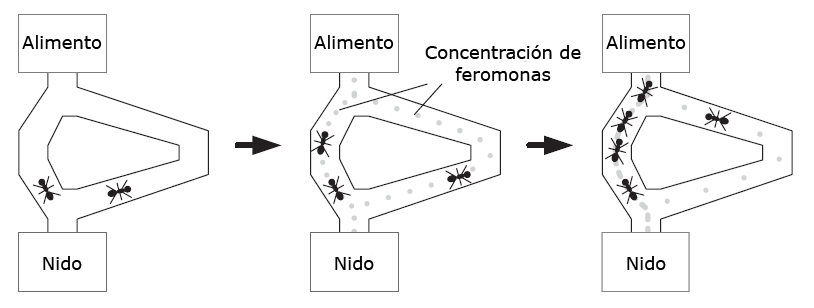
\includegraphics[scale=0.4]{./img/colonia_ejemplo.png}
	\caption{Colonia de hormigas}
	\label{img:ants}
\end{figure}

Esta feromona además tiene un factor de evaporación, esto produce que los caminos pierdan
su fuerza de atracción, cuanto más largo sea el camino, más tiempo demorará una hormiga
en recorrerlo, más se evaporará la feromona y por ende serán menos frecuentado. Por su parte
los caminos más cortos (o más óptimos) tendrán mayor cantidad de feromonas, por ende, mayor
probabilidad de ser frecuentados. Además, nos da la ventaja de evitar convergencias a optiomos locales.
Figura \ref{img:ants}.

